\documentclass[12pt]{beamer}
\newenvironment{ConCodigo}[1]
  {\begin{frame}[fragile,environment=ConCodigo]{#1}}
  {\end{frame}}
\graphicspath{{Imagenes/}{../Imagenes/}}
\usepackage[utf8]{inputenc}
\usepackage[spanish]{babel}
\usepackage{hyperref}
\usepackage{etex}
%\reserveinserts{28}
\usepackage{amsmath}
\usepackage{amsthm}
\usepackage{mathtools}
\usepackage{multicol}
\usepackage{multirow}
\usepackage{tabulary}
\usepackage{booktabs}
\usepackage{nccmath}
\usepackage{physics}
\usepackage{biblatex}
\usepackage[outdir=./]{epstopdf}
%\epstopdfsetup{outdir=./}
\usepackage{graphicx}
%\usepackage{enumitem,xcolor}
\usepackage{siunitx}
%\sisetup{scientific-notation=true}
%\usepackage{fontspec}
\usepackage{lmodern}
\usepackage{float}
\usepackage[format=hang, font=footnotesize, labelformat=parens]{caption}
\usepackage[autostyle,spanish=mexican]{csquotes}
\usepackage{standalone}
\usepackage{blkarray}
\usepackage{algorithm}
\usepackage{algorithmic}
\usepackage{tikz}
\usepackage[siunitx, RPvoltages]{circuitikz}
\usetikzlibrary{arrows,patterns,shapes}
\usetikzlibrary{decorations.markings}
\usetikzlibrary{arrows}
\usepackage{color}
\usepackage{xcolor}
%\usepackage{beton}
%\usepackage{euler}
%\usepackage[T1]{fontenc}
\usepackage[sfdefault]{roboto}  %% Option 'sfdefault' only if the base font of the document is to be sans serif
\usepackage[T1]{fontenc}
\renewcommand*\familydefault{\sfdefault}
\DeclareGraphicsExtensions{.pdf,.png,.jpg}
\usepackage{hyperref}
\renewcommand {\arraystretch}{1.5}
\newcommand{\python}{\texttt{python}}
\usefonttheme[onlymath]{serif}
\setbeamertemplate{navigation symbols}{}
\usetikzlibrary{patterns}
\usetikzlibrary{decorations.markings}
\tikzstyle{every picture}+=[remember picture,baseline]
%\tikzstyle{every node}+=[inner sep=0pt,anchor=base,
%minimum width=2.2cm,align=center,text depth=.15ex,outer sep=1.5pt]
%\tikzstyle{every path}+=[thick, rounded corners]
\setbeamertemplate{caption}[numbered]
\newcommand{\ptm}{\fontfamily{ptm}\selectfont}
%Se usa la plantilla Warsaw modificada con spruce
\mode<presentation>
{
  \usetheme{Warsaw}
  \setbeamertemplate{headline}{}
  \useoutertheme{default}
  \usecolortheme{albatross}
  \setbeamercovered{invisible}
}
% \AtBeginSection[]
% {
% \begin{frame}<beamer>{Contenido}
% \normalfont\mdseries
% \tableofcontents[currentsection]
% \end{frame}
% }

\input{../Preambulos/pre_plantilla_Warsaw_spruce}
\input{../Preambulos/pre_codigo}
\makeatletter
\setbeamercolor{section in foot}{bg=gray!30, fg=black!90!orange}
\setbeamercolor{subsection in foot}{bg=blue!30!yellow, fg=red}
\setbeamertemplate{footline}
{
  \leavevmode%
  \hbox{%
  \begin{beamercolorbox}[wd=.333333\paperwidth,ht=2.25ex,dp=1ex,center]{section in foot}%
    \usebeamerfont{section in foot} \insertsection
  \end{beamercolorbox}}%
  \begin{beamercolorbox}[wd=.333333\paperwidth,ht=2.25ex,dp=1ex,center]{subsection in foot}%
    \usebeamerfont{subsection in foot}  \insertsubsection
  \end{beamercolorbox}%
  \begin{beamercolorbox}[wd=.333333\paperwidth,ht=2.25ex,dp=1ex,right]{date in head/foot}%
    \usebeamerfont{date in head/foot} \insertshortdate{} \hspace*{2em}
    \insertframenumber{} / \inserttotalframenumber \hspace*{2ex} 
  \end{beamercolorbox}}%
  \vskip0pt%
\makeatother
\title{Funciones de interpolación con \python}
%\subtitle{Funciones de interpolación con \texttt{python}}
\author{M. en C. Gustavo Contreras Mayén}
\begin{document}
\maketitle
\fontsize{14}{14}\selectfont
\spanishdecimal{.}
\begin{frame}{Contenido}
\tableofcontents[pausesections]
\end{frame}
\section{Funciones de interpolación con \texttt{python}.}
\begin{frame}
Encontramos en \python\ una serie de funciones que permiten realizar la interpolación de un conjunto de datos, estimando la mejor aproximación, pero no debemos de confiarnos en dar por hecho que con ello, el error obtenido por la aproximación es el menor.
\\
\bigskip
La librería que debemos de utilizar es \funcionazul{scipy.interpolate}
\end{frame}
\subsection{La función \texttt{interp1d (x, y)}}
\begin{frame}
\frametitle{La función \texttt{interp1d (x, y)}}
Dentro de \funcionazul{scipy.interpolate} contamos con la función \funcionazul{interp1d} que requiere de dos argumentos - los valores de $x$ e $y$ que se utilizarán para la interpolación. 
\\
\bigskip
Se puede proporcionar un tipo de argumento opcional que especifica el tipo de procedimiento de interpolación.
\end{frame}
\begin{frame}
\frametitle{Opciones para el tipo de interpolación.}
Las opciones disponibles son:
\setbeamercolor{item projected}{bg=red!70!black,fg=white}
\setbeamertemplate{enumerate items}[circle]
\begin{enumerate}[<+->]
\item \texttt{linear}: interpola a lo largo de una línea recta entre puntos de datos vecinos.
\item \texttt{nearest}: proyecta al punto de datos más cercano.
\item \texttt{zero}: proyecta al punto de datos anterior.
\item \texttt{slinear}: usa un ``spline'' lineal.
\item \texttt{cuadratic}: usa un ``spline'' cuadrático.
\item \texttt{cubic}: usa un ``spline'' cúbico.
\end{enumerate}
\end{frame}
\begin{frame}[fragile]
El valor predeterminado de \texttt{interp1d} es una interpolación lineal. También se puede proporcionar un número entero, en cuyo caso la función utilizará un polinomio de ese orden para interpolar entre puntos. Por ejemplo:
\begin{verbatim}
F = interp1d (x, y, kind = 10)
\end{verbatim}
Utilizará un polinomio de orden 10 para interpolar entre puntos.
\end{frame}
\begin{frame}[fragile]
\frametitle{Ejemplo}
Con el siguiente código generamos un conjunto de 20 datos distribuidos entre $0$ y $10 * \pi$
\begin{lstlisting}[basicstyle=\ttfamily\normalsize, columns=fullflexible]
x = np.linspace(0, 10 * np.pi, 20)
y = np.cos(x)

#para graficar

plt.plot(x,y, 'bo', label='Datos')
\end{lstlisting}
\end{frame}
\begin{frame}
\frametitle{Resultado en la gráfica}
\begin{figure}
%\centering
\hspace*{-0.2cm}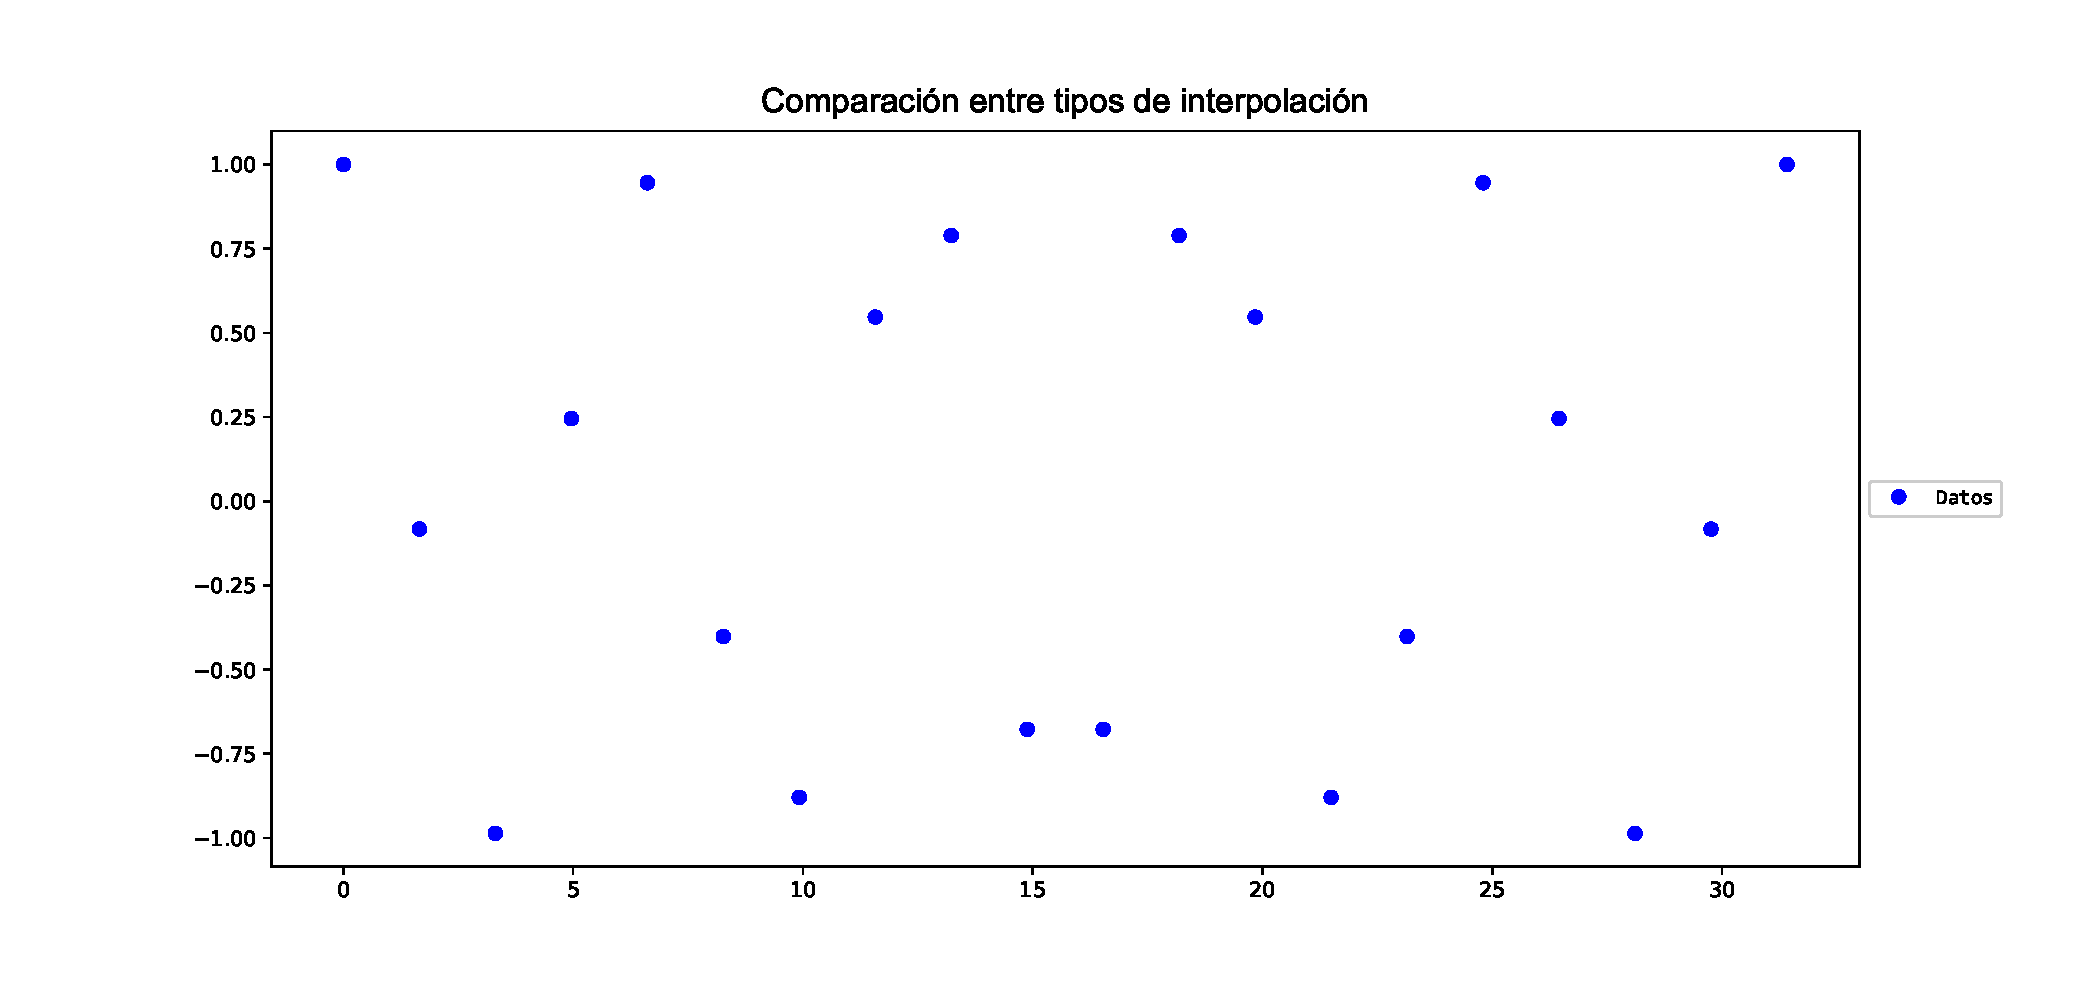
\includegraphics[scale=0.35]{interpolacion_01.eps}
\end{figure}
\end{frame}
\begin{frame}[allowframebreaks,fragile]
\frametitle{Se interpolan los datos}
\begin{lstlisting}[basicstyle=\ttfamily\normalsize, columns=fullflexible]
# Se interpolan los datos

fl = interp1d(x, y, kind='linear')

fq = interp1d(x, y, kind='quadratic')

# x.min and x.max se usan para asegurar que no
# nos salimos del intervalo de interpolacion

xint = np.linspace(x.min(), x.max(), 1000)

yintl = fl(xint)

yintq = fq(xint)

#para graficar

plt.plot(xint, yintl, label='Lineal')
plt.plot(xint, yintq, label='Cubica')
\end{lstlisting}
\end{frame}
\begin{frame}[fragile]
\frametitle{Se grafican los datos}
\begin{lstlisting}[basicstyle=\ttfamily\normalsize, columns=fullflexible]
#para graficar

plt.plot(xint, yintl, label='Lineal')

plt.plot(xint, yintq, label='Cubica')
\end{lstlisting}
\end{frame}
\begin{frame}
\frametitle{Interpolación lineal}
\begin{figure}
%\centering
\hspace*{-0.2cm}\includegraphics[scale=0.35]{interpolacion_02.eps}
\end{figure}
\end{frame}
\begin{frame}
\frametitle{Interpolación cúbica}
\begin{figure}
%\centering
\hspace*{-0.2cm}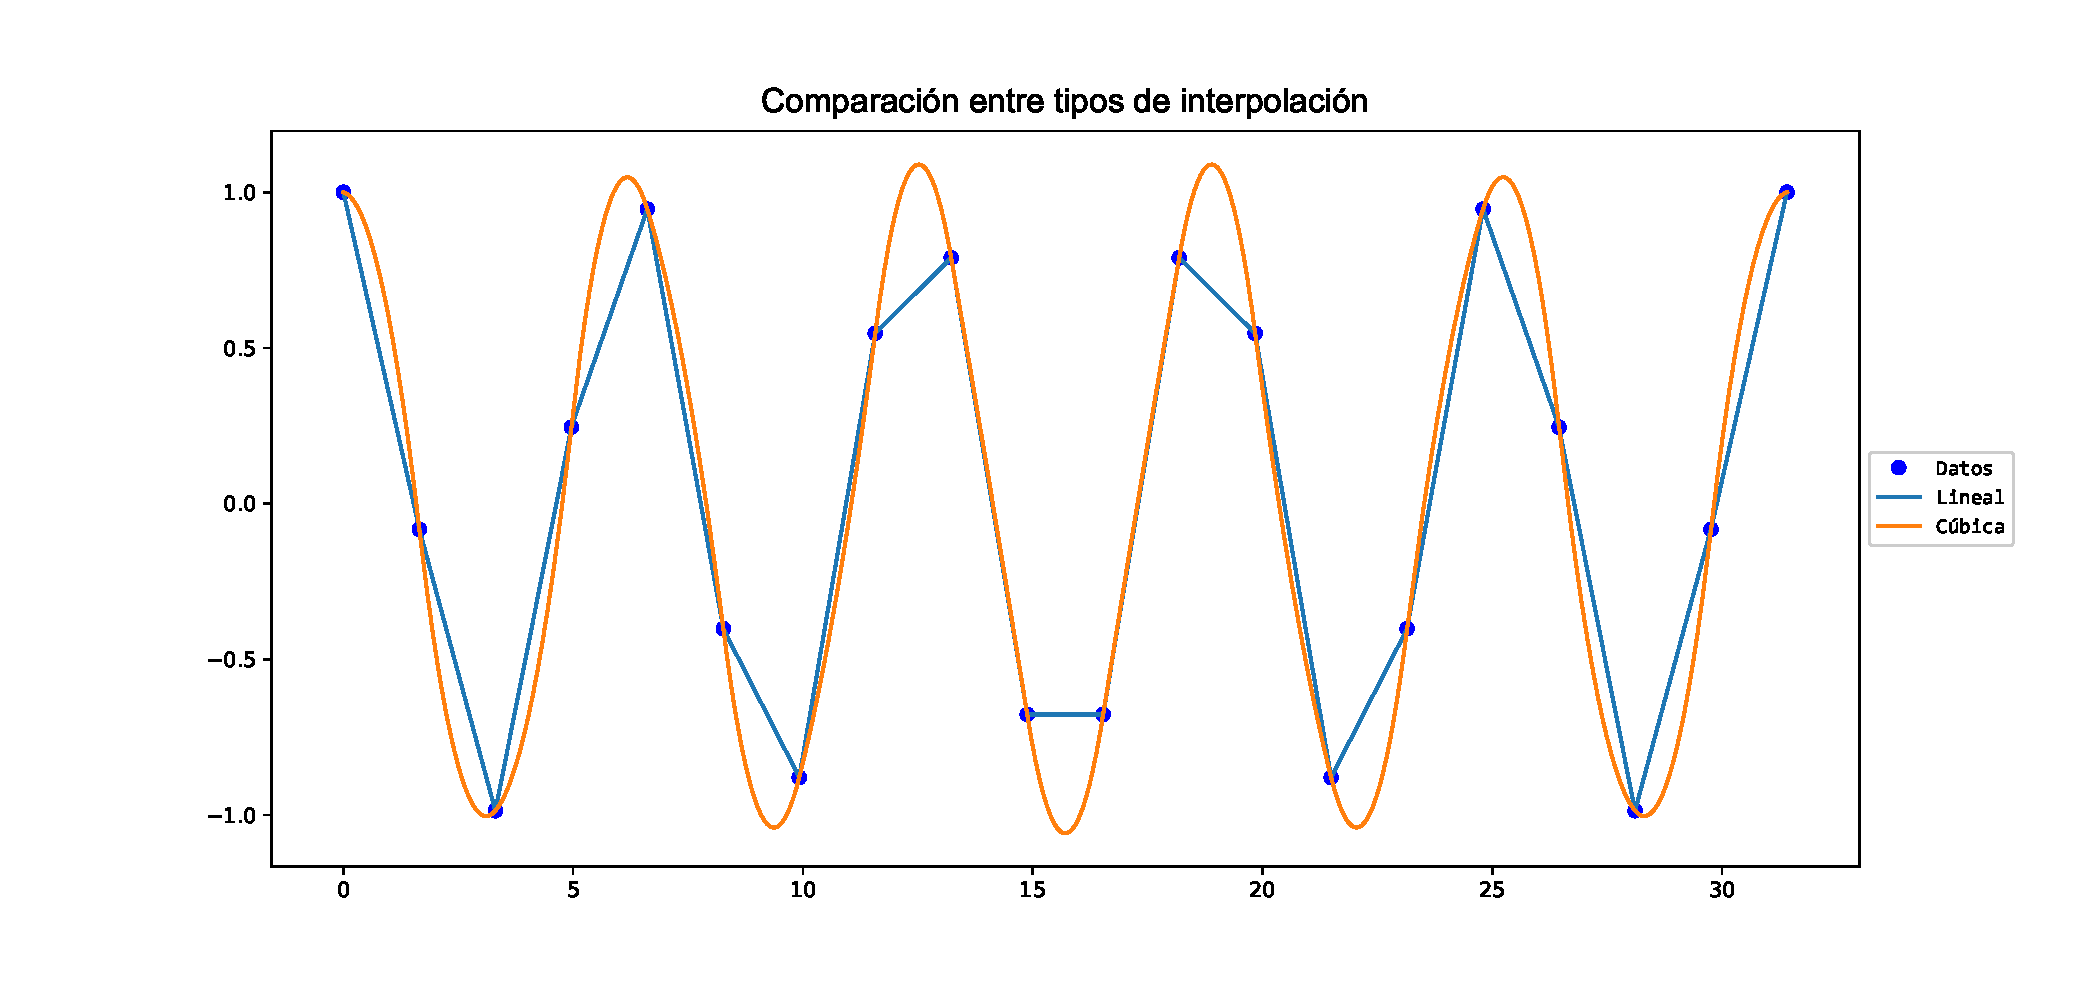
\includegraphics[scale=0.35]{interpolacion_03.eps}
\end{figure}
\end{frame}
\begin{frame}
\frametitle{Veamos otro ejemplo.}
Utilizaremos la función \texttt{sinc(x)} que está contenida dentro de la librería \texttt{numpy}.
\\
\bigskip
La función \texttt{sinc (x)}, también llamada ``función de muestreo'', es una función que se encuentra comúnmente de las teorías de procesamiento de señales y de las transformadas de Fourier.
\end{frame}
\begin{frame}
El nombre completo de la función es ``seno cardinal'', pero es comúnmente referido por su abreviatura, ``sinc''. Se define como
\[ sinc(x) = \begin{cases}
1 & \mbox{para } x = 0 \\
\dfrac{\sin x}{x} & \mbox{para cualquier otro valor} \end{cases}\]
\end{frame}
\begin{frame}[fragile]
\begin{lstlisting}[basicstyle=\ttfamily\normalsize, columns=fullflexible]
x = np.linspace(-18, 18, 36)
ruido = 0.1 * np.random.random(len(x))
senal = np.sinc(x) + ruido

interpretada = interpolate.interp1d(x, senal)
x2 = np.linspace(-18, 18, 180)
y = interpretada(x2)

cubica = interpolate.interp1d(x, senal, kind="cubic")
y2 = cubica(x2)
\end{lstlisting}
\end{frame}
\begin{frame}
\frametitle{Interpolación con la señal de muestreo}
\begin{figure}
%\centering
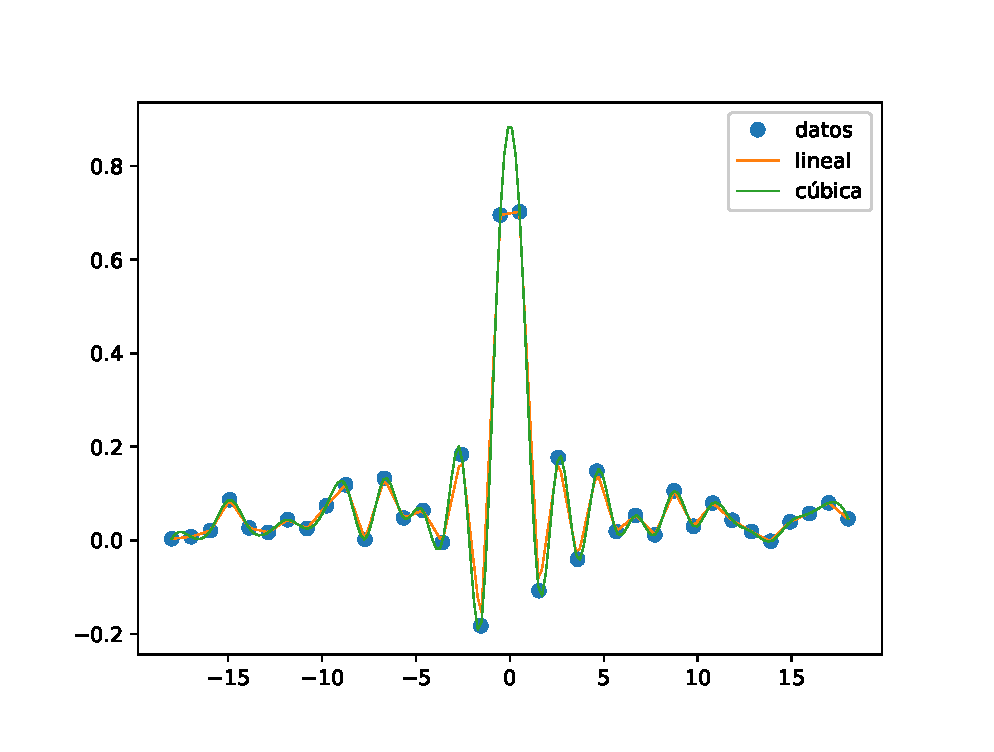
\includegraphics[scale=0.65]{interpolacion_04.eps}
\end{figure}
\end{frame}
\begin{frame}
\frametitle{Más sobre la interpolación.}
Es posible reconocer algunas características generales de la interpolación obtenida en las figuras:
\setbeamercolor{item projected}{bg=red!70!black,fg=white}
\setbeamertemplate{enumerate items}[circle]
\begin{enumerate}[<+->]
\item Las funciones de interpolación son continuas.
\item Las funciones de interpolación pasan siempre por los puntos de datos.
\item Una función cuadrática puede dar un ajuste más malo que la interpolación lineal.
\item Aumentar el orden del polinomio no siempre conduce a un mejor ajuste.
\item Las funciones de interpolación pueden oscilar drásticamente entre los puntos de datos.
\item El ajuste empeora hacia los extremos del conjunto de datos.
\end{enumerate}
\end{frame}
\begin{frame}
\frametitle{Entonces, ¿qué debo hacer al interpolar mis propios datos?}
El ``spline cúbico'' es el caballo de batalla en este terreno. Como se puede ver en la figura, proporciona una curva suave que parece ajustarse bien a los datos.
\begin{figure}
\centering
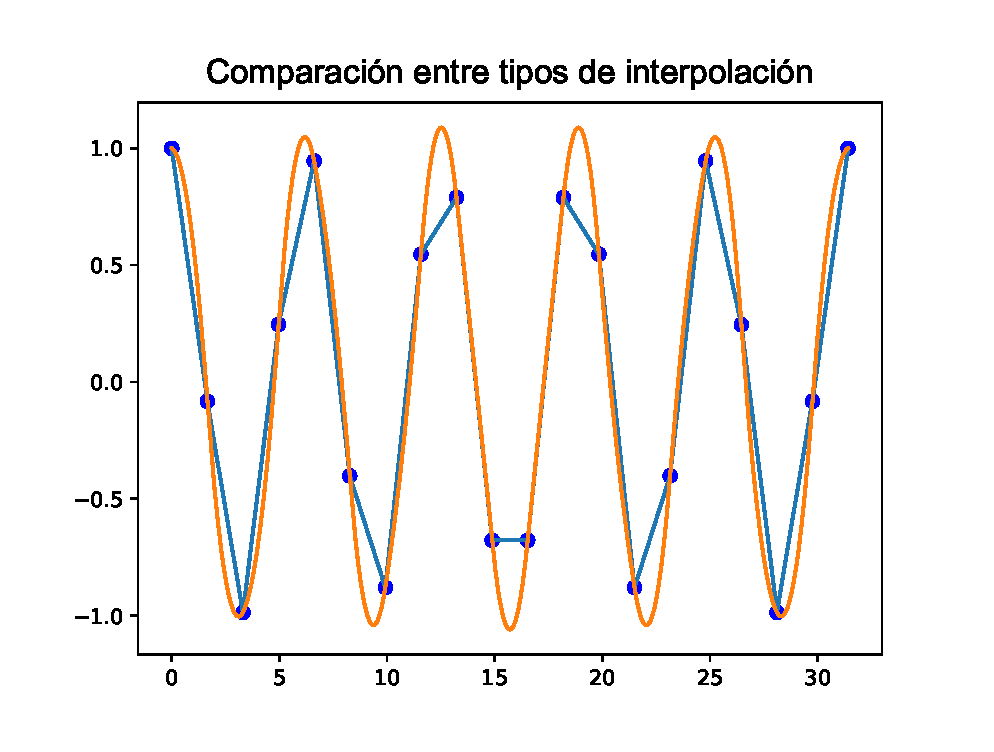
\includegraphics[scale=0.4]{interpolacion_03b.eps}
\end{figure}
\end{frame}
\begin{frame}
La suavidad se extiende más allá de lo que se ve en la gráfica: un ``spline cúbico'' tiene derivadas primera y segunda continuas.
\\
\bigskip
Esta es una propiedad útil en la física, donde las derivadas primera y segunda son bastante comunes en los análisis teóricos (leyes de Newton, ecuaciones de Maxwell, ecuación de Schröedinger, etc.)
\\
\medskip
\pause
\textcolor{blue}{Una interpolación de spline cúbico es una buena opción en la mayoría de los casos}.
\end{frame}
\begin{frame}
\frametitle{Precaución con las funciones de interpolación}
Precaución: la interpolación y la extrapolación no es lo mismo.
\\
\bigskip
Una buena función de interpolación puede ser una aproximación muy mala fuera del conjunto de puntos de datos utilizados. Por esta razón, las funciones generadas por \texttt{interp1d (x, y)} ni siquiera devolverán un número cuando proporcione un valor de la variable independiente fuera del rango del conjunto de datos: se obtiene un \texttt{ValueError} en su lugar.
\end{frame}
\section{Fenómeno de Runge}
\begin{frame}
\frametitle{Fenónemo de Runge}
Hasta el momento hemos revisado un par de estrategias para calcular un polinomio que pase por un conjunto de datos $(x_{i}, y_{i})$, pero hay que considerar un efecto importante al respecto: no siempre el mejor polinomio será aquel el de mayor grado $n$.
\\
\medskip
Veamos el siguiente ejemplo: sea la función:
\[ f(x) = \dfrac{1}{1 + 25 x^{2}}\]
\end{frame}
\begin{frame}
\frametitle{Gráfica de la función $f(x)$}
\begin{figure}
	\centering
	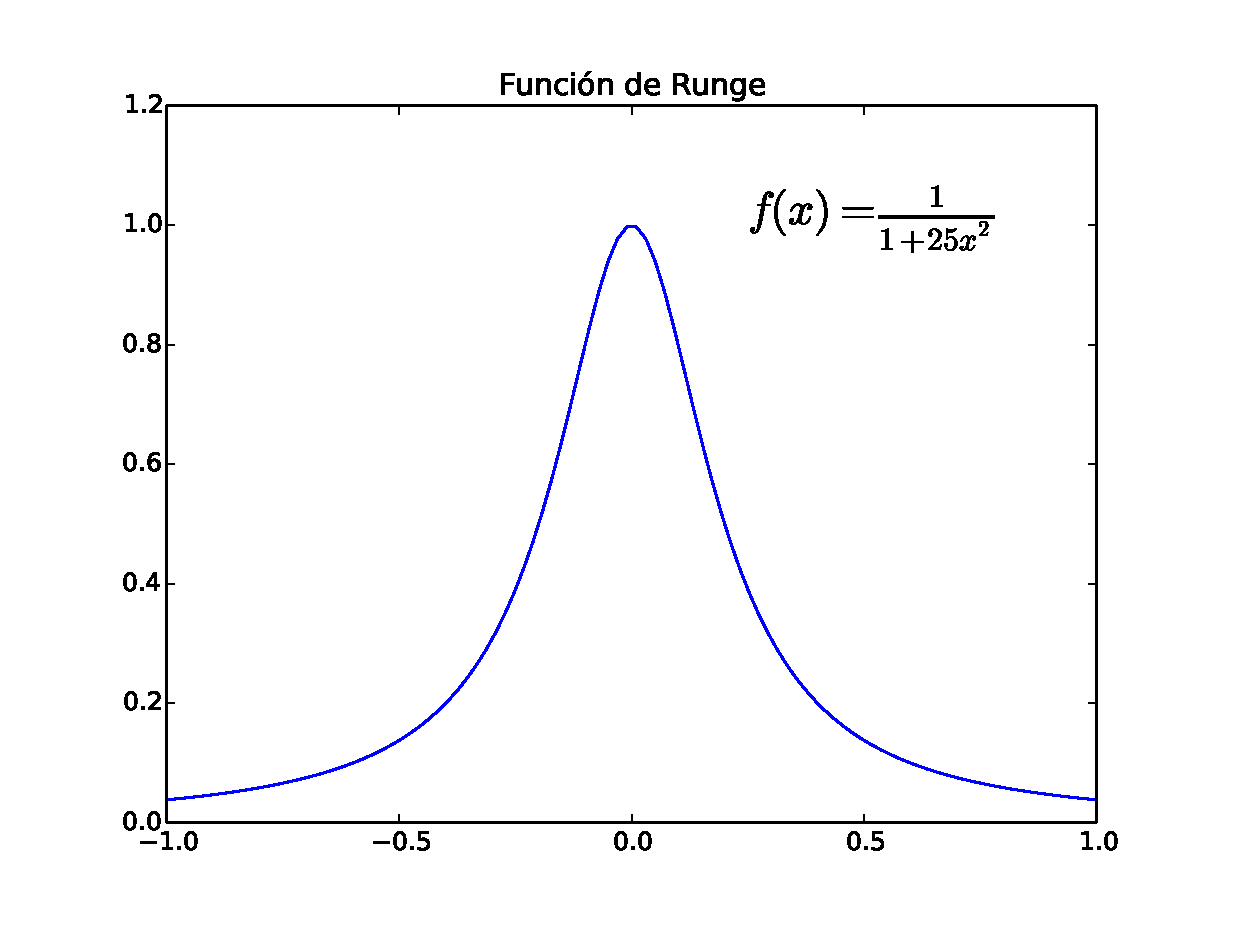
\includegraphics[scale=0.5]{Imagenes/Funcion_Runge_01.eps} 
\end{figure}
\end{frame}
\begin{frame}
\frametitle{Elección de puntos para interpolar}
\begin{figure}
	\centering
	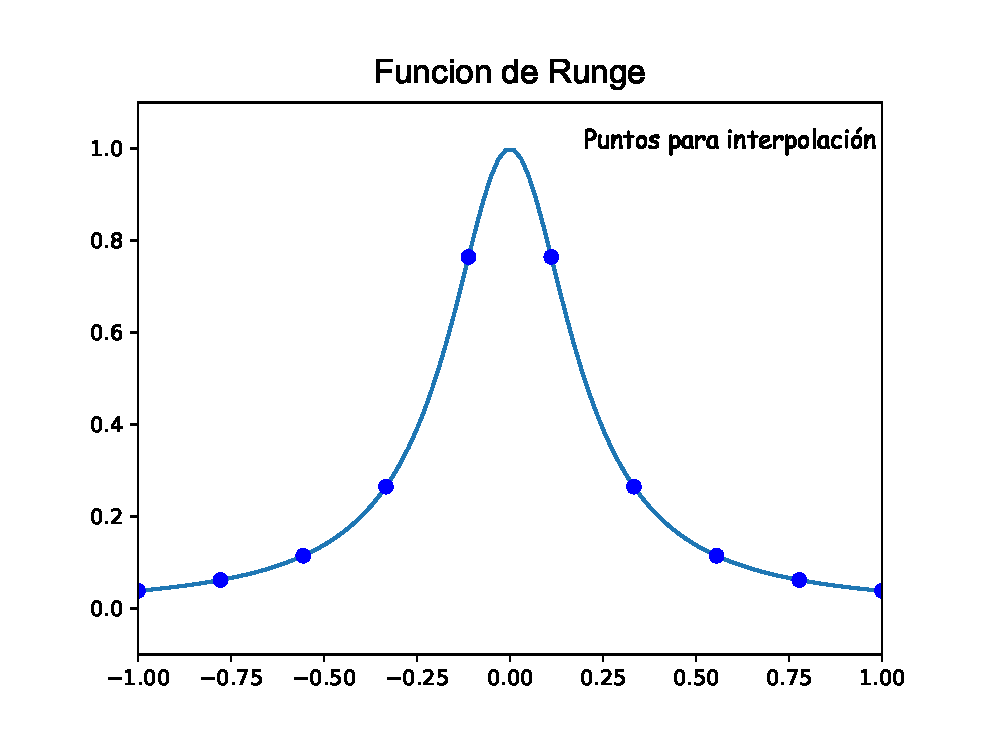
\includegraphics[scale=0.5]{Imagenes/Funcion_Runge_2017_01.eps} 
\end{figure}
\end{frame}
\begin{frame}
\frametitle{Interpolación con Lagrange}
Interpolando los puntos con Lagrange.
\begin{figure}
	\centering
	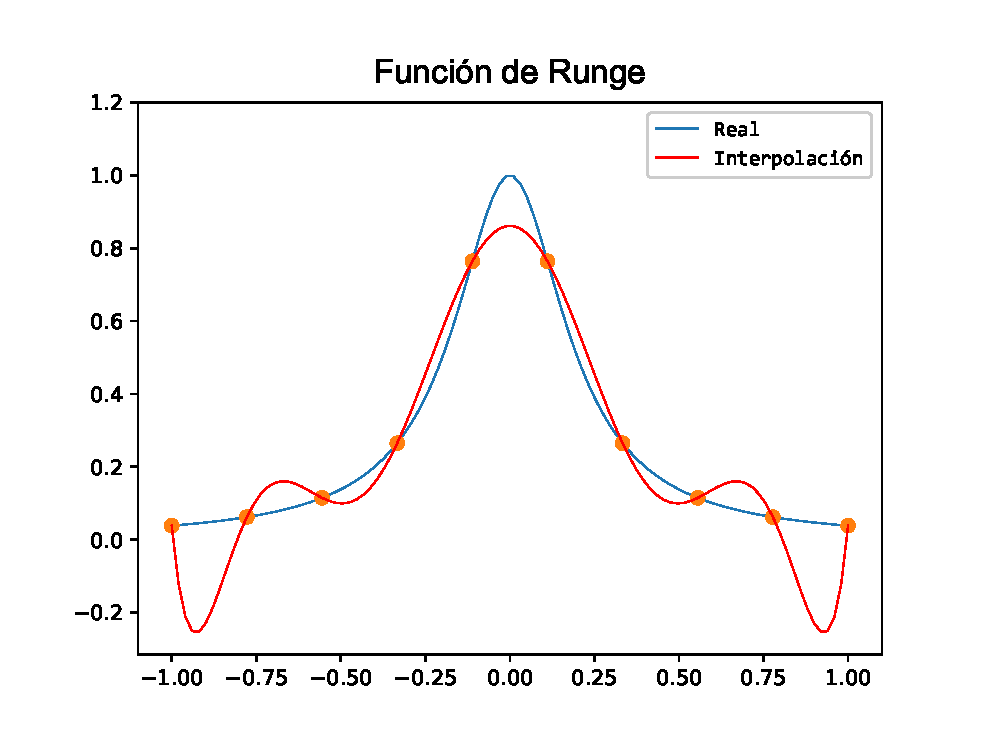
\includegraphics[scale=0.5]{Imagenes/Funcion_Runge_2017_02.eps} 
\end{figure}
\end{frame}
\begin{frame}
\frametitle{¿Qué hacemos al respecto?}
Como hemos visto en la gráfica anterior, la función que resulta del proceso de interpolación ``oscila'' a través de los puntos que deseamos interpolar; aquí el caso es que si aumentamos el grado del polinomio, los resultados serán aún más indeseables.
\\
\medskip
La pregunta obligada es: ¿qué podemos hacer para mejorar la interpolación?
\end{frame}
\subsection{Uso de splines}
\begin{frame}
\frametitle{¿Qué es un spline?}
En términos nada riguroso, se puede decir que un spline es una función definida por una familia de polinomios ``sociables'', donde el término sociable se usa para indicar que los polinomios que constituyen una función spline, están estrechamente vinculados.
\\
\medskip
El nombre de \emph{spline}, viene del inglés ya que es un instrumento que utilizaban los ingenieros navales para dibujar curvas suaves, forzadas a pasar por un conjunto de puntos prefijados.
\end{frame}
\begin{frame}
\frametitle{Las tres B's de los splines}
El uso de las funciones splines tiene mucha aceptación y popularidad se deben a tres razones básicas:
\setbeamercolor{item projected}{bg=red!70!black,fg=white}
\setbeamertemplate{enumerate items}[circle]
\begin{enumerate}[<+->]
\item \textbf{Buenos:} Se  pueden usar en la solución de una gran variedad de problemas.
\item \textbf{Baratos:} Ya que su cálculo es muy sencillo y económico.
\item \textbf{Bonitos:} La teoría matemática en que se basan es muy simple y a la vez elegante.
\end{enumerate}
\end{frame}
\begin{frame}
\frametitle{Manejando splines con \python}
Usaremos la librería \texttt{scipy} que contiene varias funciones con las que ahorramos tiempo para manejar splines y ajustar funciones sociables a un conjunto de datos.
\\
\medskip
No está de más que revises la teoría al respecto, en la mayoría de los libros de análisis numérico, podrás encontrar la construcción matemática y formal de los splines.
\end{frame}
\begin{frame}
\frametitle{Funciones para los splines}
Necesitaremos de dos pasos para el uso de splines con \python, de la libería: \texttt{scipy.interpolate}, las cuales son:
\begin{enumerate}
\item \textbf{splrep}: Calcula el spline básico (B-spline) para una curva 1-D.
\\
\medskip
Dados un conjunto de puntos $(x[i],y[i])$ determina una aproximación con un spline suave de grado $k$ en el intervalo $xb \leq x \leq xe$.
\item \textbf{splev}: Evalúa un B-spline o sus derivadas. Dados los nodos y coeficientes de un B-spline, calcula el valor del polinomio suave y sus derivadas.
\end{enumerate}
\end{frame}
\begin{frame}[allowframebreaks, fragile]
\frametitle{Código}
\begin{lstlisting}[basicstyle=\ttfamily\normalsize, columns=fullflexible]
import matplotlib.pyplot as plt
import scipy.interpolate as si
from numpy import *

x = linspace(-1, 1, 100)
y = 1./(1 + 25 * x**2)

def trazador_cub(n):
    xi = linspace(-1, 1, n)
    yi = 1./(1 + 25 * xi**2)
    tck = si.splrep(xi, yi)
    return tck
\end{lstlisting}
\end{frame}
\begin{frame}[allowframebreaks, fragile]
\frametitle{Código}
\begin{lstlisting}[basicstyle=\ttfamily\normalsize, columns=fullflexible]
tck = trazador_cub(8)
ys8 = si.splev(x, tck)

tck = trazador_cub(12)
ys12 = si.splev(x, tck)

plt.plot(x, y)
plt.plot(x, ys8,'+g-', label='n=8')
plt.plot(x, ys12,'+r-',label ='n=12')
plt.legend(loc='best')
plt.title('Interpolacion con splines cubicos')
plt.ylim(-0.2, 1.2)
plt.show()
\end{lstlisting}
\end{frame}
\begin{frame}
\frametitle{Resultados gráficos}
\begin{figure}
	\centering
	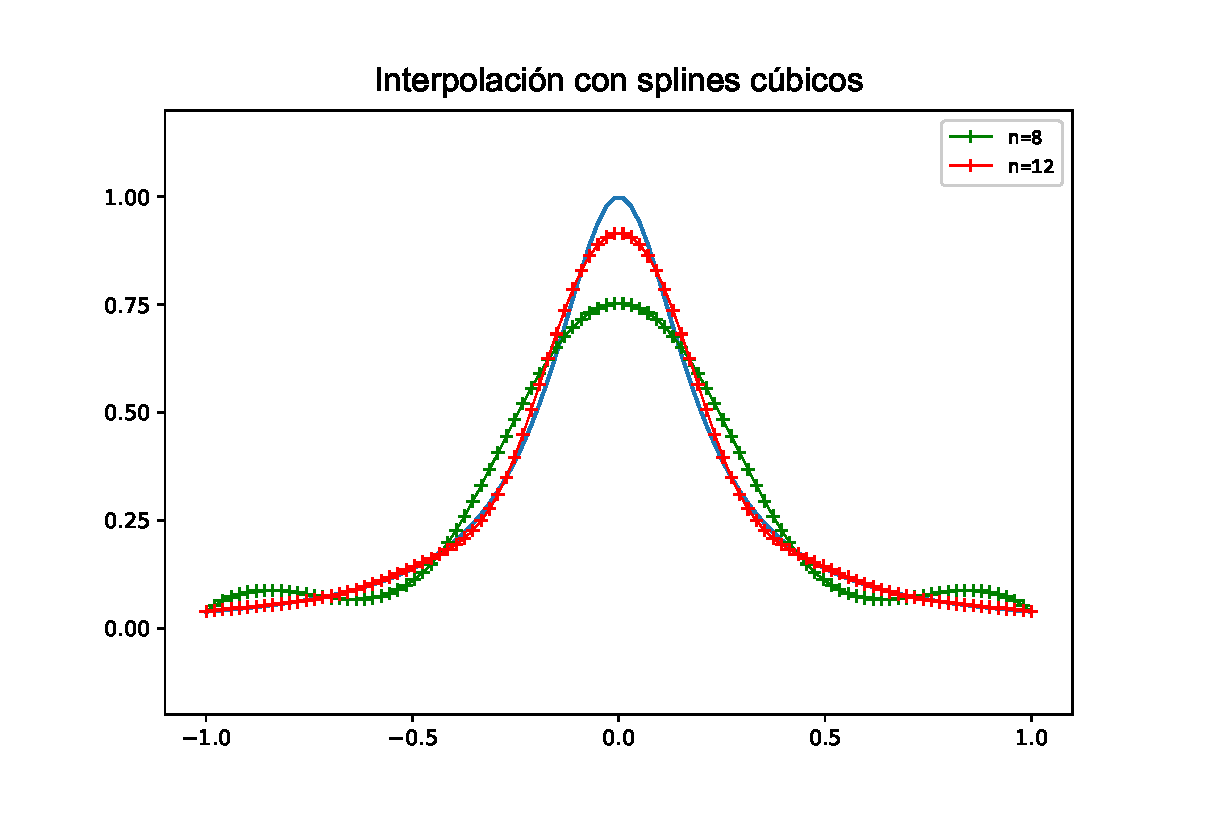
\includegraphics[scale=0.5]{Imagenes/Funcion_Runge_2017_03.eps} 
\end{figure}
\end{frame}
% \section{Cálculo de raíces}
% \begin{frame}
% \frametitle{Cálculo de raíces}
% Sea $y= f(x)$.  Los valores de $x$ que hacen que $y=0$ se
% denominan \textcolor{blue}{raíces de la ecuación}.
% \\
% \bigskip
% El teorema fundamental del álgebra indica que todo polinomio de grado $n$, tiene $n$ raíces. En el caso de las raíces reales, se tiene que corresponden a los valores $x$ que hacen que la función corte el eje de las abscisas:
% \end{frame}
% \begin{frame}
% \frametitle{Ejemplo de la función seno(x)}
% \begin{figure}
% 	\centering
% 	\includegraphics[scale=0.4]{raices00.eps} 
% \end{figure}
% \end{frame}
% \begin{frame}
% Las raíces de un polinomio pueden ser reales o complejas.
% \\
% \bigskip
% Si un polinomio tiene coeficientes reales
% \[ a_{0},a_{1},a_{2},\ldots,a_{n-1},a_{n} \]
% entonces todas las raíces complejas siempre ocurrirán en pares conjugados complejos.
% \end{frame}
% \begin{frame}
% Por ejemplo, un polinomio cúbico tiene la siguiente
% forma general:
% \[ f(x)= a_{0}x^{3}+a_{1}x^{2}+a_{2}x+a_{3}\]
% \setbeamercolor{item projected}{bg=red!70!black,fg=white}
% \setbeamertemplate{enumerate items}[circle]
% \begin{enumerate}
% \item Tres raíces reales distintas.
% \item Una raíz real con multiplicidad 3.
% \item Una raíz real simple y una raíz real con multiplicidad 2.
% \item Una raíz real y un par conjugado complejo.
% \end{enumerate}
% \end{frame}
% \begin{frame}[fragile]
% \frametitle{Tres raíces distintas}
% \begin{minipage}{5cm}
% \fontsize{12}{12}\selectfont
% \[ \begin{split}
% f(x)=& x^{3} - 3x^{2}-x+3 \\
% =& (x-3)(x+1)(x-1)
% \end{split} \]
% Las raíces son:
% \[ \begin{split}
% x_{1} =& 3 \\
% x_{2} =& -1 \\
% x_{3} =& 1 \\
% \end{split}\]
% \end{minipage}
% \hspace{0.5cm}
% \begin{minipage}{4.5cm}
% \begin{figure}
% 	\centering
% 	\includegraphics[scale=0.3]{raices01.eps} 
% \end{figure}
% \end{minipage}
% \end{frame}
% \begin{frame}[fragile]
% \frametitle{Raíz real con multiplicidad 3}
% \begin{minipage}{5cm}
% \fontsize{12}{12}\selectfont
% \[ \begin{split}
% f(x)=& x^{3} - 6x^{2} + 12x - 8 \\
% =& (x-2)^{3}
% \end{split} \]
% Las raíces son:
% \[ \begin{split}
% x_{1} =& 2 \\
% x_{2} =& 2 \\
% x_{3} =& 2 \\
% \end{split}\]
% \end{minipage}
% \hspace{0.5cm}
% \begin{minipage}{4.5cm}
% \begin{figure}
% 	\centering
% 	\includegraphics[scale=0.3]{raices02.eps} 
% \end{figure}
% \end{minipage}
% \end{frame}
% \begin{frame}[fragile]
% \frametitle{Raíz real simple y \\ una raíz real con multiplicidad 2}
% \begin{minipage}{5cm}
% \fontsize{12}{12}\selectfont
% \[ \begin{split}
% f(x)=& x^{3} - 12x + 16 \\
% =& (x+4)(x-2)^{2}
% \end{split} \]
% Las raíces son:
% \[ \begin{split}
% x_{1} =& -4 \\
% x_{2} =& 2 \\
% x_{3} =& 2 \\
% \end{split}\]
% \end{minipage}
% \hspace{0.5cm}
% \begin{minipage}{4.5cm}
% \begin{figure}
% 	\centering
% 	\includegraphics[scale=0.3]{raices03.eps} 
% \end{figure}
% \end{minipage}
% \end{frame}
% \begin{frame}[fragile]
% \frametitle{Raíz real y un par conjugado complejo}
% \begin{minipage}{5cm}
% \fontsize{12}{12}\selectfont
% \[ \begin{split}
% f(x)=& x^{3} - 2x^{2}- 3x +10  \\
% =& (x+2)(x- (2+i))* {}\\
% *& (x-(2-i))
% \end{split} \]
% Las raíces son:
% \[ \begin{split}
% x_{1} =& -2 \\
% x_{2} =& 2+i \\
% x_{3} =& 2-i \\
% \end{split}\]
% \end{minipage}
% \hspace{0.5cm}
% \begin{minipage}{4.5cm}
% \begin{figure}
% 	\centering
% 	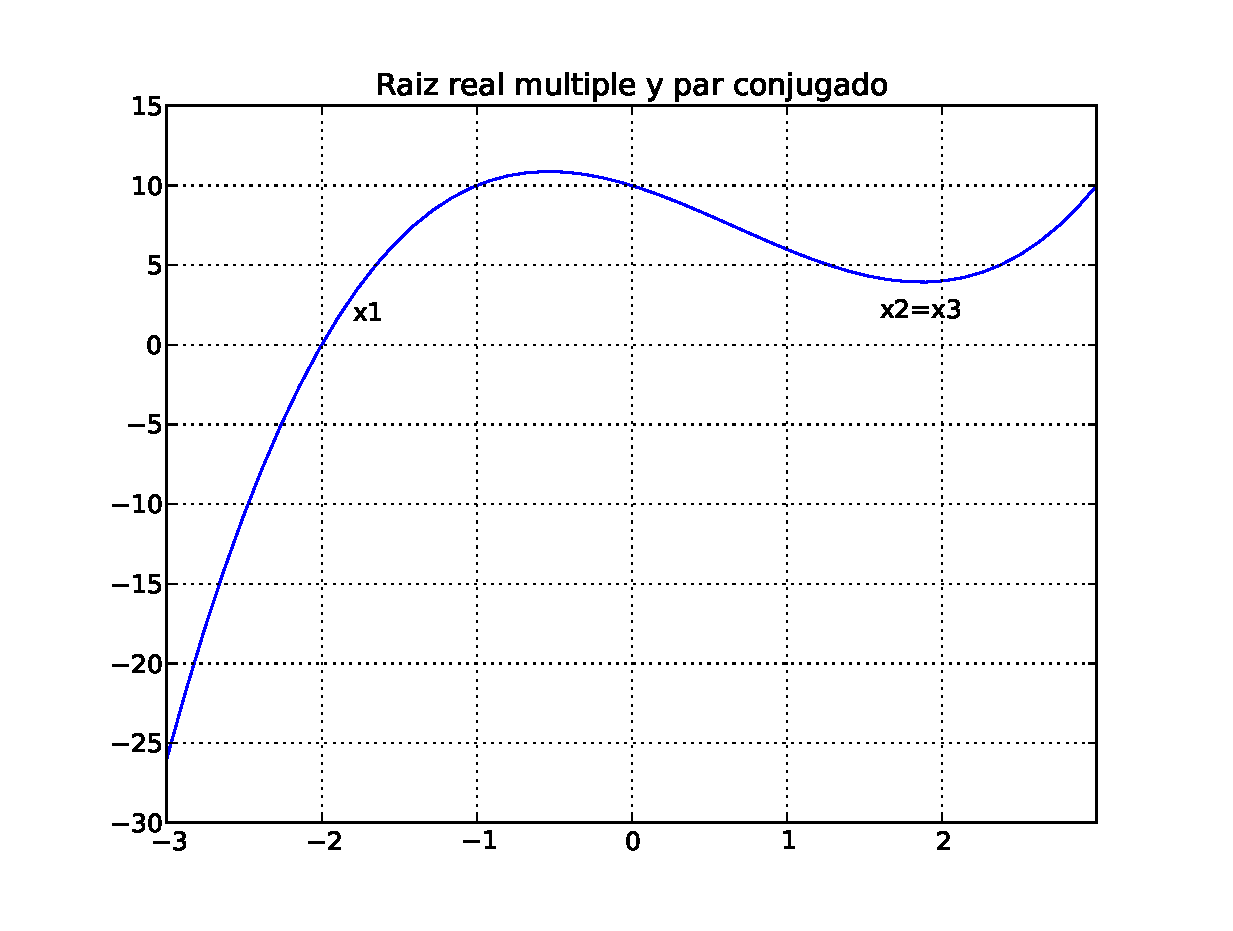
\includegraphics[scale=0.3]{raices04.eps} 
% \end{figure}
% \end{minipage}
% \end{frame}
% \section{Funciones algebraicas}
% \begin{frame}
% \frametitle{Funciones algebraicas}
% Sea $g=f(x)$ la función expresada como
% \[ f_{n}y^{n} + f_{n-1}y^{n-1} + \ldots + f_{1}y + f_{0} = 0 \]
% Donde $f_{i}$ es un polinomio de orden $i$ en $x$.
% \\
% \bigskip
% Los polinomios son un caso simple de funciones algebraicas que se representan generalmente como
% \[f_{n}(x) = a_{0} + a_{1}x + a_{2} x^{2}+ \ldots +a_{n}x^{n} \]
% Donde $n$ es el orden del polinomio.
% \end{frame}
% \section{Funciones trascendentales}
% \begin{frame}
% \frametitle{Funciones trascedentales}
% Son aquellas que no son algebraicas.
% \\
% \bigskip
% Comprenden a las funciones trigonométricas, exponenciales, logarítmicas, entre otras.
% \\
% \bigskip
% Ejemplos:
% \begin{itemize}
% \item \[ f(x)=ln(x^{2}-1) \]
% \item \[g(x)=e^{-0.2x} \sin(3x-5) \]
% \end{itemize}
% \end{frame}
% \begin{frame}
% Los métodos numéricos estándar para encontrar
% raíces pueden clasificarse en dos rubros:
% \\
% \bigskip
% \textbf{1.} La determinación de las raíces reales de ecuaciones algebraicas y trascendentales. Las técnicas a emplear en estos casos se diseñaron con el fin de encontrar el valor de una raíz simple de acuerdo con un conocimiento previo de su posición aproximada.
% \end{frame}
% \begin{frame}
% \textbf{2.} La determinación de todas las raíces reales y complejas de un polinomio, para lo cual los métodos numéricos estén diseñados específicamente para polinomios. 
% \\
% \bigskip
% Determinan sistemáticamente todas las raíces del polinomio en lugar de hacerlo sólo con una, dada la posición aproximada.
% \end{frame}
% \section{Método de incrementos sucesivos}
% \begin{frame}
% \frametitle{Método de incrementos sucesivos}
% Podemos aproximar mucho mejor las raíces de una función, cuando la graficamos.
% \\
% \bigskip
% Con una gráfica general de unos cuantos puntos, tendríamos lo necesario para considerar los valores de las raíces.
% \\
% \bigskip
% El método de búsqueda incremental es una herramienta útil que podemos adoptar en conjunto con otras estrategias de cálculo de raíces, por sí sólo, éste método no nos ofrece más que una referencia sobre en dónde podrían estar esas raíces.
% \end{frame}
% \begin{frame}
% La idea básica detrás del método de búsqueda incremental es simple: si $f(x_{1})$ y $f(x_{2})$ tienen signos opuestos, entonces hay al menos una raíz en el intervalo $(x_{1}, x_{2})$.
% \end{frame}
% \begin{frame}[fragile]
% \frametitle{Caso en donde es posible encontrar la raíz}
% \begin{center}
% 	\begin{tikzpicture}[font=\footnotesize, scale=1.3]
% 		\draw[<->](0,0) -- (6,0);
% 		\draw[<->](3,-2) -- (3,2);
% 		\draw [red] (0.5,1.5) .. controls (2,0.2) and (4,-1) .. (5.5,-1.5);
% 		\draw[dashed] (1,0) -- (1,1.1);
% 		\draw (0.9,-0.2) node {a}; 
% 		\draw (1.2,1.4) node {f(a)};
% 		\draw[dashed] (5,0) -- (5,-1.33);
% 		\draw (5,0.2) node {b}; 
% 		\draw (5,-1.7) node {f(b)};
% 		\draw(4.5,1.5) node {$f(a)*f(b)<0$};
% 	\end{tikzpicture}
% \end{center}
% \end{frame}
% \begin{frame}
% \frametitle{Caso en donde no es posible encontrar la raíz}
% \begin{center}
% 	\begin{tikzpicture}[font=\footnotesize, scale=1.3]
% 		\draw[<->](0,0) -- (6,0);
% 		\draw[<->](3,-1) -- (3,3);
% 		\draw [red] (0.5,2.5) .. controls (2.5,0.5) and (3.5,0.5) .. (5.5,2.5);
% 		\draw [dashed] (1,0) -- (1,2.1);
% 		\draw (1,-0.2) node {a};
% 		\draw (1.1,2.2) node {f(a)};
% 		\draw [dashed] (4.5,0) -- (4.5,1.65);
% 		\draw (4.5,-0.2) node {b};
% 		\draw (4.5, 2) node {f(b)};
% 		\draw (5,3.5) node {$f(a)*f(b)>0$};
% 	\end{tikzpicture}
% \end{center}
% \end{frame}
% \begin{frame}
% Si el intervalo es lo suficientemente pequeño, es probable que contenga una sola raíz. Así, los ceros de $f(x)$ puede ser detectados mediante la evaluación de la función a intervalos $\Delta x$ y mirando cuando se presente un cambio de signo en la función.
% \end{frame}
% \begin{frame}
% Hay varios problemas con el método de búsqueda incremental:
% \setbeamercolor{item projected}{bg=red!70!black,fg=white}
% \setbeamertemplate{enumerate items}[circle]
% \begin{enumerate}[<+->]
% \item Es posible perder dos raíces muy próximas entre sí, si el incremento de búsqueda $\Delta x$ es mayor que la separación de las raíces.
% \item Una raíz doble (dos raíces que coinciden) no será detectada.
% \item Algunas singularidades de $f(x)$ se puede confundir con raíces. Por ejemplo, $f(x) = \tan x$. Tiene cambios de signo en $x = \pm 1/2 n\pi$ con $n = 1, 3, 5,\ldots$
% \end{enumerate}
% \end{frame}
% \begin{frame}
% Estos puntos no son ceros verdaderos, ya que la función no cruza el eje $x$.
% \begin{figure}
% 	\centering
% 	\includegraphics[scale=0.4]{raices05.eps} 
% \end{figure}
% \end{frame}
% \subsection{Código Método de incrementos sucesivos}
% \begin{frame}
% \frametitle{Código Método de incrementos sucesivos}
% El código busca un cero de la función $f$ que proporciona el usuario en el intervalo
% $(a,b)$ en incrementos de $dx$.
% \\
% \bigskip
% Se devuelve el intervalo $(x_{1}, x_{2})$ donde se encuentra la raíz, si la búsqueda
% se ha realizado correctamente; se devuelve $x_{1} = x_{2} = \mathsf{None}$ cuando no se encontraron raíces.
% \\
% \bigskip
% Luego de que se encontró la primera raíz, (la más cercana al punto $a$), se puede llamar de nuevo al procedimiento, sustitiyendo $x_{2}$ con el fin de encontrar la siguiente raíz. Esto se puede repetir siempre y cuando se detecta una raíz.
% \end{frame}
% \begin{frame}[fragile]
% \begin{lstlisting}[basicstyle=\ttfamily\normalsize, columns=fullflexible]
% def buscaraiz(f,a,b,dx):
%     x1 = a; f1 = f(a)
%     x2 = a + dx; f2 = f(x2)
%     while f1*f2 > 0.0:
%         if x1 >= b: return None
%         x1 = x2; f1 = f2
%         x2 = x1 + dx; f2 = f(x2)
%     else:
%         return x1,x2
% \end{lstlisting}
% \end{frame}
% \begin{frame}
% \frametitle{Ejemplo}
% Usa el método de incrementos sucesivos y con $\Delta x= 0.2$, para estimar la raíz con el valor positivo más pequeño de la función:
% \[ f(x) = x^{3} - 10 x^{2} + 5\]
% \end{frame}
% \begin{frame}
% \frametitle{Revisión general de la función}
% Conviene graficar inicialmente la función para tener una idea sobre los intervalos iniciales, \emph{evita proponer valores del intervalo muy cercanos a la raíz}, lo que se busca es que revises la implementación del código.
% \begin{figure}
% 	\centering
% 	\includegraphics[scale=0.4]{Imagenes/funcion_raiz_01.eps} 
% \end{figure}
% \end{frame}
% \begin{frame}
% \frametitle{Consideraciones importantes.}
% Si al momento de graficar la función para explorar un poco, notamos que de izquierda a derecha tenemos las tres raíces $x_{0}, x_{1}, x_{2}$, aunque aún no sabemos su valor, podemos estimar en qué intervalo se encuentran.
% \\
% \bigskip
% El algoritmo de incrementos sucesivos debería de informarnos en qué intervalos se encuentran las raíces.
% \end{frame}
% \begin{frame}
% \frametitle{Raíces del polinomio}
% El problema pide calcular la raíz positiva más pequeña del polinomio de tercer grado, de acuerdo a la gráfica, la raíz buscada es $x_{1}$, ya que $x_{0}<0$ y $x_{2} > x_{1}$.
% \begin{figure}
% 	\centering
% 	\includegraphics[scale=0.5]{funcion_raiz_02.eps} 
% \end{figure}
% \end{frame}
% \begin{frame}
% \frametitle{Intervalo de inicio}
% Con toda tranquilidad presentamos el intervalo de inicio para el método de incrementos sucesivos para determinar el intervalo en donde se encuentra $x_{1}$: la raíz positiva más pequeña de $f(x)$.
% \begin{figure}
% 	\centering
% 	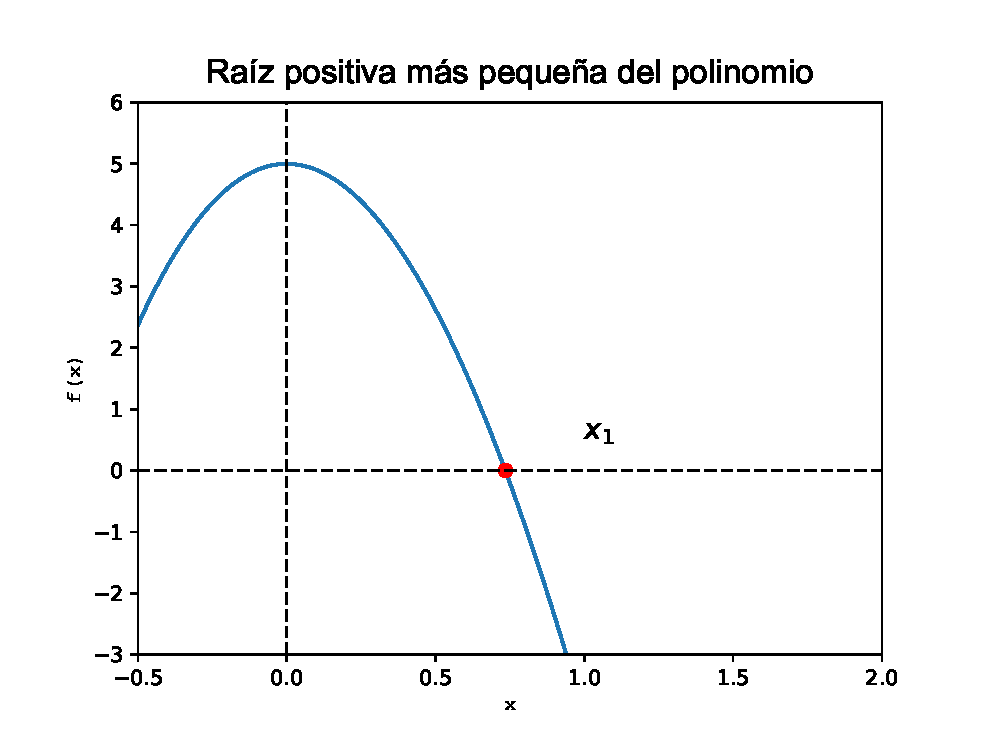
\includegraphics[scale=0.5]{funcion_raiz_03.eps} 
% \end{figure}
% \end{frame}

% \begin{frame}[fragile]
% \begin{lstlisting}[basicstyle=\ttfamily\normalsize, columns=fullflexible]
% def f(x): return x**3 - 10*x**2 + 5.

% a, b, dx = (0.0,1.5, 0.2)

% print ('El intervalo es: ')
% x1, x2 = buscaraiz(f,a,b,dx)
% print (x1,x2)
% \end{lstlisting}
% \end{frame}
% \begin{frame}
% El código incluye el intervalo $[0.0, 1,5]$, pero una vez que localiza que ya no hay cambio de signo, se detiene.
% \\
% \bigskip
% ¿Cómo podríamos mejorar nuestro código para que sin importar el valor inicial del intervalo, realice un ``escaneo'' sobre todo el eje de las abscisas? De tal manera que nos reporte el total de raíces que existen y en los intervalos en dónde se encuentran. (Tomando en cuenta que usaríamos un intervalo inicial razonable)
% \end{frame}
\end{document}